\addtocontents{toc}{\protect\setcounter{tocdepth}{2}}
\chapter{Fases previas a la construcción de la aplicación}
\graphicspath{{imagenes/estructura_y_desarrollo/}}

La temporalidad del proyecto no es exacta del todo ya que los puntos 3.1 y 3.2 se hicieron aquellos dos primeros meses de prácticas extracurriculares mientras que los otros son totalmente nuevos.
\\Para el seguimiento de las fases y tareas se han estado utilizado la herramienta Trello y las nuevas funcionalidades de GitHub que incorpora tableros parecidos a los de Trello.

\section{Reuniones iniciales con los clientes}

La reunión inicial fue con Juan Francisco Sanjuan Estrada donde me explicó los distintos objetivos que se tenía pensado para la aplicación y los puntos de vista de los técnicos. La organización, gestión y préstamos del inventario se realizaba mediante la utilización de hojas de cálculo.
\\Dentro de las hojas de cálculo se hacía un detallado exhaustivo del objeto y también se indicaba su ubicación actual dentro del Edificio Científico Técnico III.
\\El problema es que esto no estaba tan organizado como parecía en un principio debido a que la gestión no la realizaba únicamente un técnico sino que eran tres. Es decir, había tres filosofías distintas a la hora de ir gestionando una parte dle inventariado del Departamento de Informática.
\\Después de estas aclaraciones Juan me comentó que no tenían un diseño en mente en el Departamento por lo que las propuestas iniciales de diseño iban a ser libres siempre y cuando se satisfacieran los requisitos principales de esta como la adición y eliminación del inventario y la concesión de préstamos.
\\\\Luego de esta primera reunión acordamos en que podría visualizar los archivos Excel de los técnicos. Estos me compartieron sus ficheros y desde ahí pude empezar a realizar la definición de los diferentes campos que irían ligados a cada tabla en la base de datos. Desde esa primera definición de campos se haría una propuesta inicial.
\\La propuesta inicial fue esta:

\begin{figure}\resizebox{
    \linewidth}{!}{
    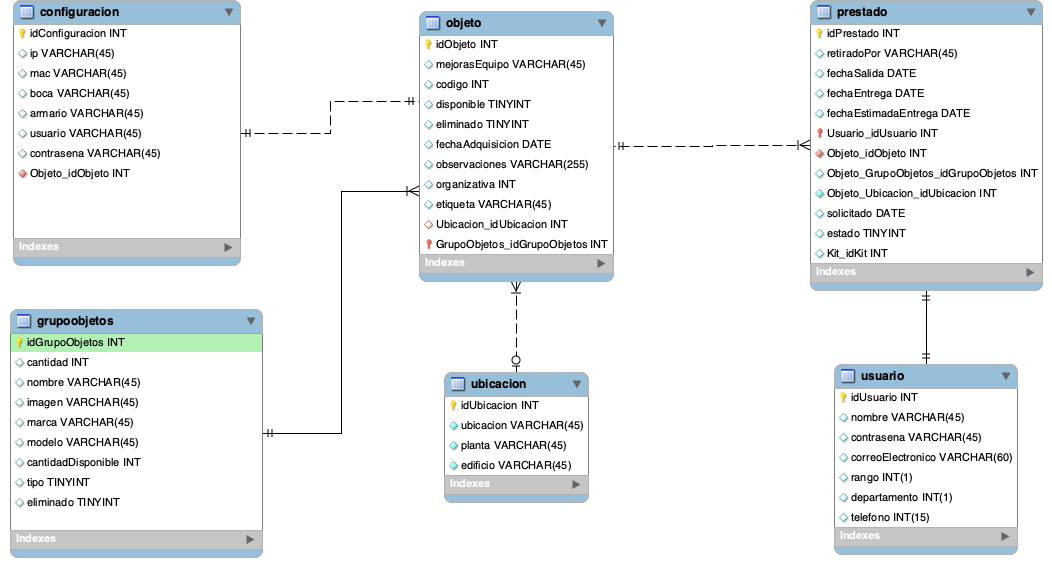
\includegraphics{db_old_design.png}
    }
    \caption{Diseño principal de la base de datos}
\end{figure}

La lógica de la aplicación consistiría en generar un grupoobjetos de un determinado tipo, inventario o fungible, 1 o 0. Dentro de este se contendrían objetos que irían vinculados a una ubicación. También los objetos irían vinculados a una posible configuración.
\\Esta configuración ¿para qué sirviría? Resulta que los técnicos aparte de manejar el inventariado disponible en la universidad también manejan las claves y accesos a esos determinados objetos, como puede ser el armario donde se ubiquen, sus direcciones mac o ip, las bocas de conexión con las regletas y más.
\\Este objeto tendría la posibilidad de tener varios préstamos, aunque es verdad que sería uno activo por persona, siempre dejando un registro de los anteriores usos que se hayan realizado del mismo. Este préstamo tendría que ir ligado obligatoriamente a un usuario. Contiene un campo de ``retiradoPor'' en el caso de que un docente o investigador quiera realizar un préstamo para su alumno.
\\\\La propuesta inicial fue aceptada por el grupo de los técnicos y por el director del proyecto así que podíamos continuar hacia adelante. Más adelante se realizaron unas modificaciones en los datos que manejarían los objetos por lo que las columnas de la tabla son las definitivas.
\\Preparé las propuestas iniciales de diseño mediante la utilización de la herramiento de Adobe XD. El aprendizaje de la herramienta es rápido y fácil de usar, aparte de que ya la había empezado a utilizar unos años atrás. Adobe XD le dió un toque de frescura y profesionalidad a las propuestas de diseño.
\\Las propuestas iniciales fueron ligadas a un diseño móvil ya que desde el primer momento se buscó que fuera responsive el sitio web. Esto influyó luego a la hora de realizar el diseño ya que se basó en un funcionamientos de ``cards'', es decir, componentes web con forma de carta y con fácil adaptabilidad a diseños móviles.
\\El esquema de navegación de la propuesta inicial nos quedaría tal que así:

\begin{figure}\resizebox{
    \linewidth}{!}{
    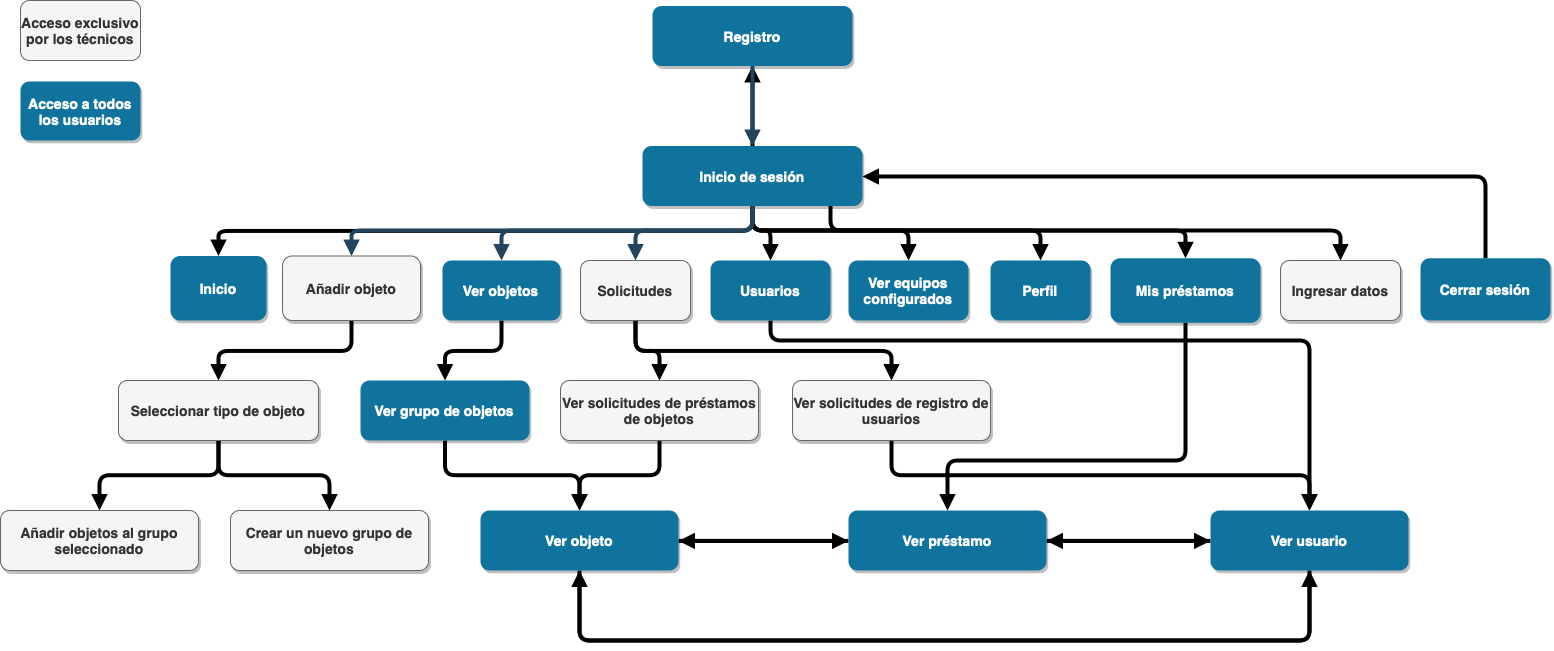
\includegraphics{flujo_de_navegacion.png}
    }
    \caption{Diseño principal del sistema de navegación}
\end{figure}

\subsection{Inicio de sesión y registro}

El registro del usuario no conllevaba un registro instantáneo del mismo ya que este tiene que ser dado de alta por un técnico del sistema.

\begin{figure}
    \begin{center}
        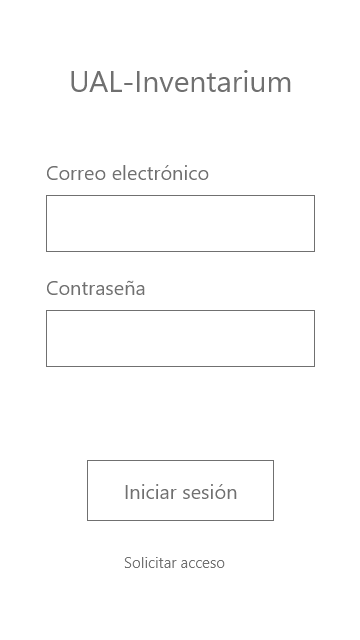
\includegraphics[scale=0.5]{web_design_adobe_xd/inicio_de_sesion.png}
        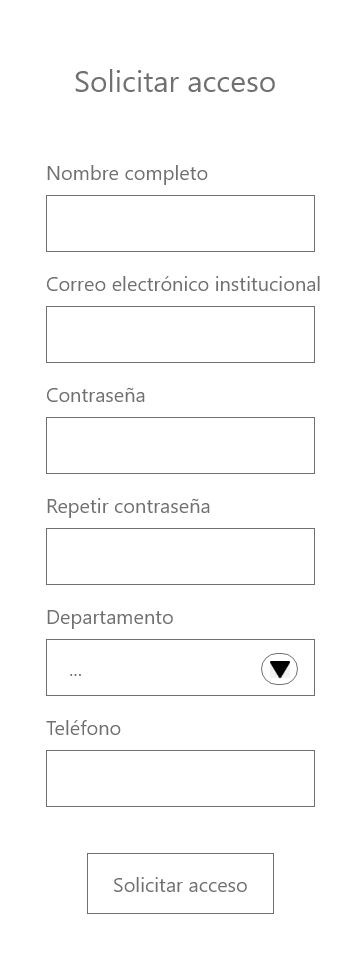
\includegraphics[scale=0.4]{web_design_adobe_xd/registro.png}
        \caption{Diseño del inicio de sesión y del registro}
    \end{center}
\end{figure}

Dentro del inicio de sesión vemos un campo interesante a considerar y es el de departamento. Una de las solicitudes que hizo el director del proyecto era poder agrupar a los usuarios dentro de departamentos. En este caso refiriéndose a dentro del personal docente e investigador que pertenecen al Departamento de Informática.
\\Los valores del departamento en la base de datos pueden ser los siguientes:

\begin{itemize}
    \item 0 = Departamento de informática (valor por defecto)
    \item 1 = Ingeniería de sistemas y automática
    \item 2 = Lenguaje y sistemas informáticos
    \item 3 = Ciencias de la computación e inteligencia artificial
    \item 4 = Arquitectura y tecnología de computadores
\end{itemize}

Otro campo para comprobar es el del correo electrónica institucional teniendo que ser este con la extensión \textbf{@inlumine.ual.es} o \textbf{@ual.es}.

\subsection{Barra de navegación}

La barra de navegación vertical tuvo una pequeña modificación que era incorporar una pequeña sección de inicio donde aparecieran información pertinente y relevante para el usuario. Esto será explicado más adelante en la parte de desarrollo.

\begin{figure}
    \begin{center}
        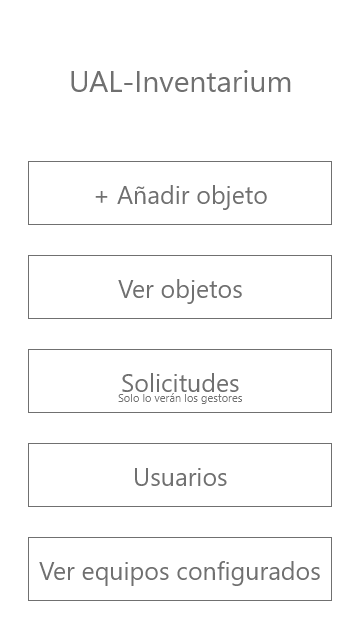
\includegraphics[scale=0.5]{web_design_adobe_xd/menu_principal.png}
        \caption{Diseño de la barra lateral de búsqueda}
    \end{center}
\end{figure}

Dentro de ella podemos ver cinco apartados que derivan en varios componentes visuales:

\begin{itemize}
    \item Añadir objeto: un acceso rápido donde poder añadir objetos dentro de grupos de objetos. Sección de menú solo visible para los técnicos.
    \item Ver objetos: apartado donde se visualizan los grupos de objetos, que contienen tanto el inventariado, fungibles y kits.
    \item Solicitudes: un menú donde se visualizan las solicitudes tanto de alta de usuarios como de objetos que le puedan llegar a los técnicos.
    \item Usuarios: componente visual donde cargan los usuarios registrados que hay dentro de la aplicación.
    \item Ver equipos configurados: aquí cargan únicamente objetos a los que se les haya aplicado una configuración. En caso de que no, no aparecerían.
\end{itemize}

\subsection{Añadir objeto}

\begin{figure}
    \begin{center}
        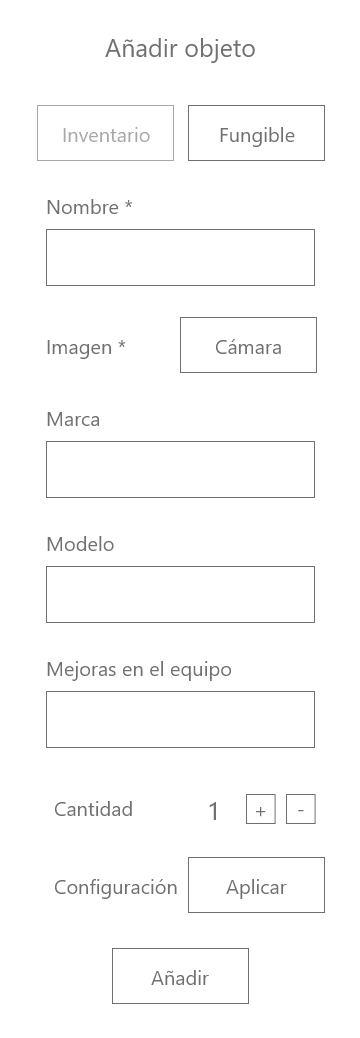
\includegraphics[scale=0.5]{web_design_adobe_xd/add_fungible.png}
        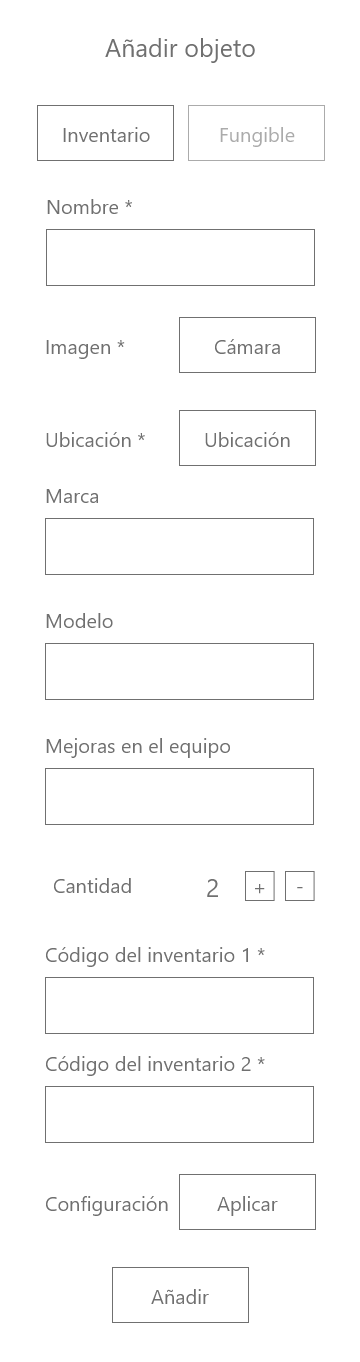
\includegraphics[scale=0.4]{web_design_adobe_xd/add_inventario.png}
        \caption{Diseño de la característica para poder añadir fungibles e inventarios}
    \end{center}
\end{figure}

La única diferencia entre añadir un objeto de tipo inventario y otro fungible es que en el de inventario hay que registrar su código. Siempre que vayamos a añadir uno de estos elementos tiene que ser dentro de un \textbf{grupo de objetos} que debemos haber creado anteriormente. Por el resto son los dos idénticos y se le puede añadir el mismo tipo de información.
\\No solamente tenemos fungibles e inventarios sino que también tenemos kits.
\\Un \textbf{kit} podemos considerarlo como otro nivel de agrupación. Ya que un kit contiene más objetos dentro suyo que llamaremos ``objetos kit''. Para entender los niveles de agrupación aquí tenéis un esquema explicándolas.

\begin{figure}\resizebox{
    \linewidth}{!}{
    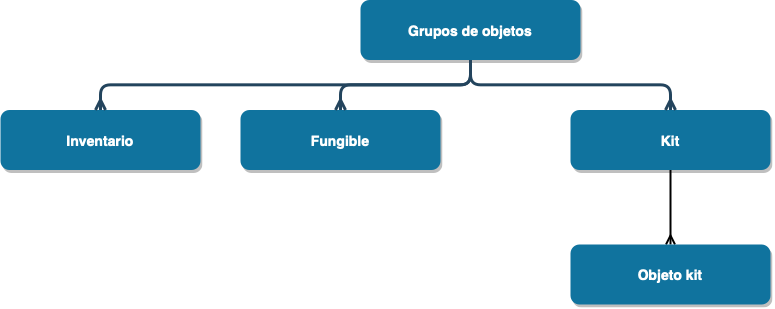
\includegraphics{jerarquia_grupo_objetos.png}
    }
    \caption{Jerarquía de elementos que derivan de grupo de objetos}
\end{figure}

\subsection{Grupo de objetos y objetos}

Dentro de la sección de ``ver objetos'' dentro de la barra de navegación esta nos llevará a la visualización de los grupos de objetos de la aplicación. Dentro de las cuales contendrán objetos. Estos dos conjuntos se pueden modificar y además se pueden pedir solicitudes para los objetos.

\begin{figure}
    \begin{center}
        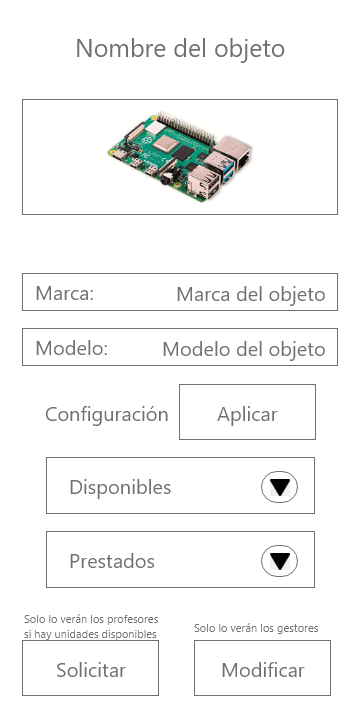
\includegraphics[scale=0.4]{web_design_adobe_xd/grupo_objetos.png}
        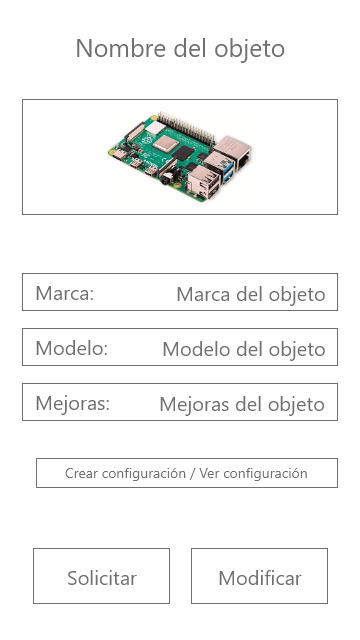
\includegraphics[scale=0.4]{web_design_adobe_xd/objeto_disponible.png}
        \caption{Grupo de objetos a la izquierda y objetos que contiene a la derecha}
    \end{center}
\end{figure}
\section{Planificación y elaboración del desarrollo del proyecto}

Esta sección implica dos apartados de relevante importancia.

\subsection{Redacción del proyecto}

Para la redacción del proyecto como se ha explicado anteriormente está utilizandose la herramienta LaTeX. Esta serie de archivos viene incorporado al repositorio principal del proyecto dentro de una carpeta llamada documentación.
\\Nuestra carpeta de documentación a la vez está subdividida en varios apartados:

\subsubsection{Build}
Carpeta que viene por defecto incorporada dentro de la ``compilación'' del proyecto que realiza LaTeX. Dentro de ella se genera el documento PDF que gracias a Visual Studio Code se va generando cada vez que se guarda un archivo del proyecto que vaya ligado o afecte al main.tex

\subsubsection{Bibliografía}
En este apartado se añadirá la bibliografía utilizada durante la realización del proyecto.

\subsubsection{Capítulos}
Dentro de esta carpeta se guardarán cada uno de los capitulos del documento. En el caso de que un capítulo presente apartados demasiados extensos se generará una carpeta con el nombre del capítulo y se meterán las secciones dentro de este. Gracias a hacer esto la modificación de cada zona del documento se hace de una forma mucho más cómoda.

\subsubsection{Diagramas}
Aquí se almacenan los diagramas del proyecto. Estos pueden estar en archivos de imágenes aunque también pueden estar generados mediante LaTeX. Debido a la unicidad que presentan los diagramas estos no están separados en diferentes carpetas por cada capítulo que haya.

\subsubsection{Imágenes}
Como su propio nombre indica se almacenan las imágenes del proyecto. Estas generalmente están divididas por carpetas con el nombre de los capítulos. En el caso de que sea demasiado extensa también se contempla la posibilidad de realizar el almacenaje mediante secciones.

\subsubsection{Include}
Aquí se añadirán los archivos que generen inclusiones dentro de nuestro documento. Dependiendo de para qué sean estos añadidos irán con unas determinadas agrupaciones u otras.

\subsubsection{main.tex}
Esto no es un directorio pero es un archivo de relevancia. Su contenido es escaso debido a la generalización que se presenta en la disposición de la documentación. Dentro de él se pueden encontrar las inclusiones al principio del documento. La adición del índice, los capítulos y de la bibliografía al final de la página. Es el archivo que utiliza LaTeX para generar nuestro documento PDF.


\subsection{Elaboración del desarrollo del proyecto}

Esta sección consiste en la explicación y descomposición de pasos que se realizará para la elaboración de la aplicación. Una vez hecha la lógica de la aplicación, su dominio y sus casos de uso se procederá a la maquetación del sistema.

\subsubsection{Generación de la base de datos}

Generación de la base de datos, para ello se utilizará MariaDB.

\subsubsection{Construcción de la Interfaz de Programación de Aplicaciones (API)}
La creación de la API debe realizarse de forma cuidadosa, ya que tiene que incorporar todas las reglas de negocio y cualquier paso adicional que haya que añadir en cada una de las peticiones. Estos pueden consistir, por ejemplo, en que cuando un objeto es creado hay que sumar una unidad dentro del campo de ``objetos'' y ``objetosDisponibles'' de su respectivo grupo de objetos.

\subsubsection{Construcción de la aplicación}
Se detallarán cada uno de los pasos más adelante debido a que la construcción de esta depende en pequeña medida al framework utilizado que en este caso es Angular. En todo caso el orden de creación de ficheros sería:
\begin{enumerate}
    \item Creación de interfaces.
    \item Creación de servicios.
    \item Creación de componentes visuales.
\end{enumerate}
\section{Preparación del entorno de trabajo}

Como decía Robert Owen, un reconocido empresario galés, en el siglo XVIII:

\begin{displayquote}
    Mejorando el entorno se mejora al hombre.
\end{displayquote}

El desarrollo de esta preparación previa ha supuesto un ahorro de tiempo bastante grande para el proyecto.
\\Esta sección irá estructurada en consonancia a la cronología de creación de cada parte del entorno. Empezando por la semilla de todo: Github.

\subsection{GitHub}
El proyecto se realizará en GitHub. Esto se hace de forma muy rápida y fácil.

\begin{enumerate}
    \item Hay que dirigirse a la dirección de \url{github.com}. Donde podrá observarse algo parecido a la figura \ref{pagina_principal_github}.
          \begin{figure}[htbp]
              \centering
              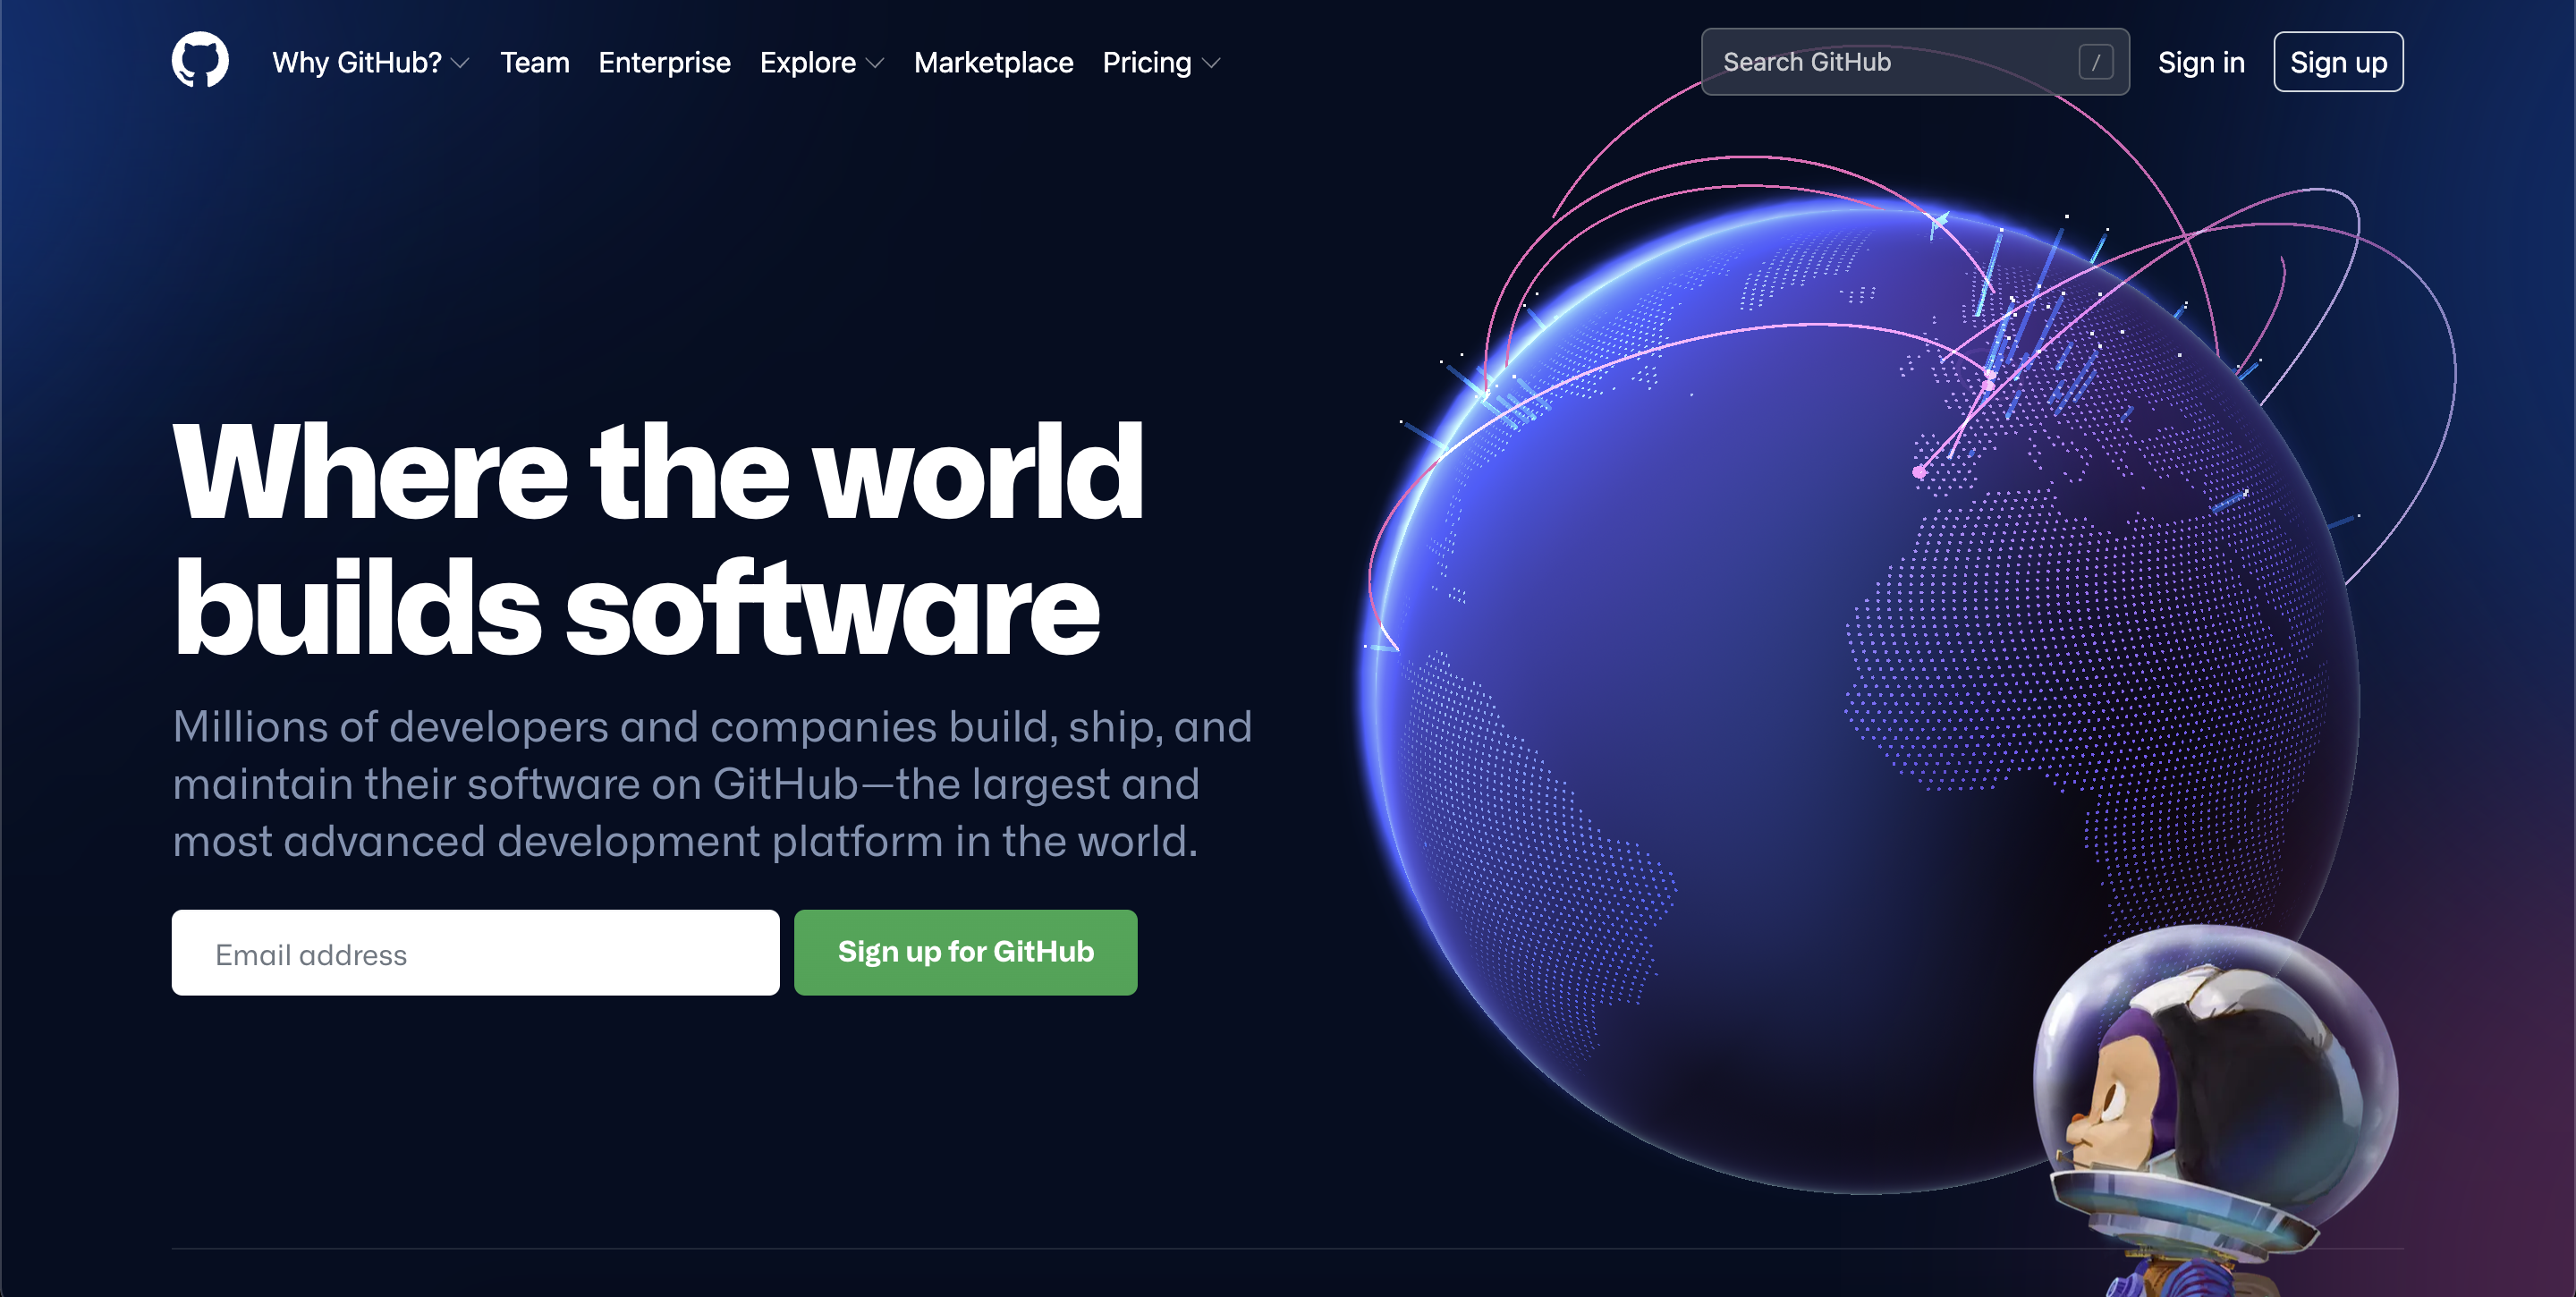
\includegraphics[scale=0.3]{preparacion_entorno/pagina_principal_github.png}
              \caption{Página principal de GitHub}\label{pagina_principal_github}
          \end{figure}
    \item En la parte superior derecha aparecerá ``Sign up'' donde se clicará para poder registrarse dentro de la web.
    \item Una vez se haya realizado el registro se volverá a \url{github.com} y se clicará a la izquierda de ``Sign up'' que pone ``Sign in'' donde podrá iniciarse sesión.
    \item Cuando se haya iniciado sesión hay que dirigirse a la parte superior izquierda clicando en ``new'' para crear un nuevo repositorio.
    \item Se rellenarán los campos que se solicitan para crear un nuevo repositorio. Se le dará el nombre de Inventarium al repositorio y se marcará en la casilla para que sea privado. También se procederá a añadirle un archivo del tipo Readme para poder describir partes del proyecto dentro de este. Por último se pulsará sobre el botón ``Create repository'' como puede verse en la figura \ref{creando_repositorio_github}.
          \begin{figure}[htbp]
              \centering
              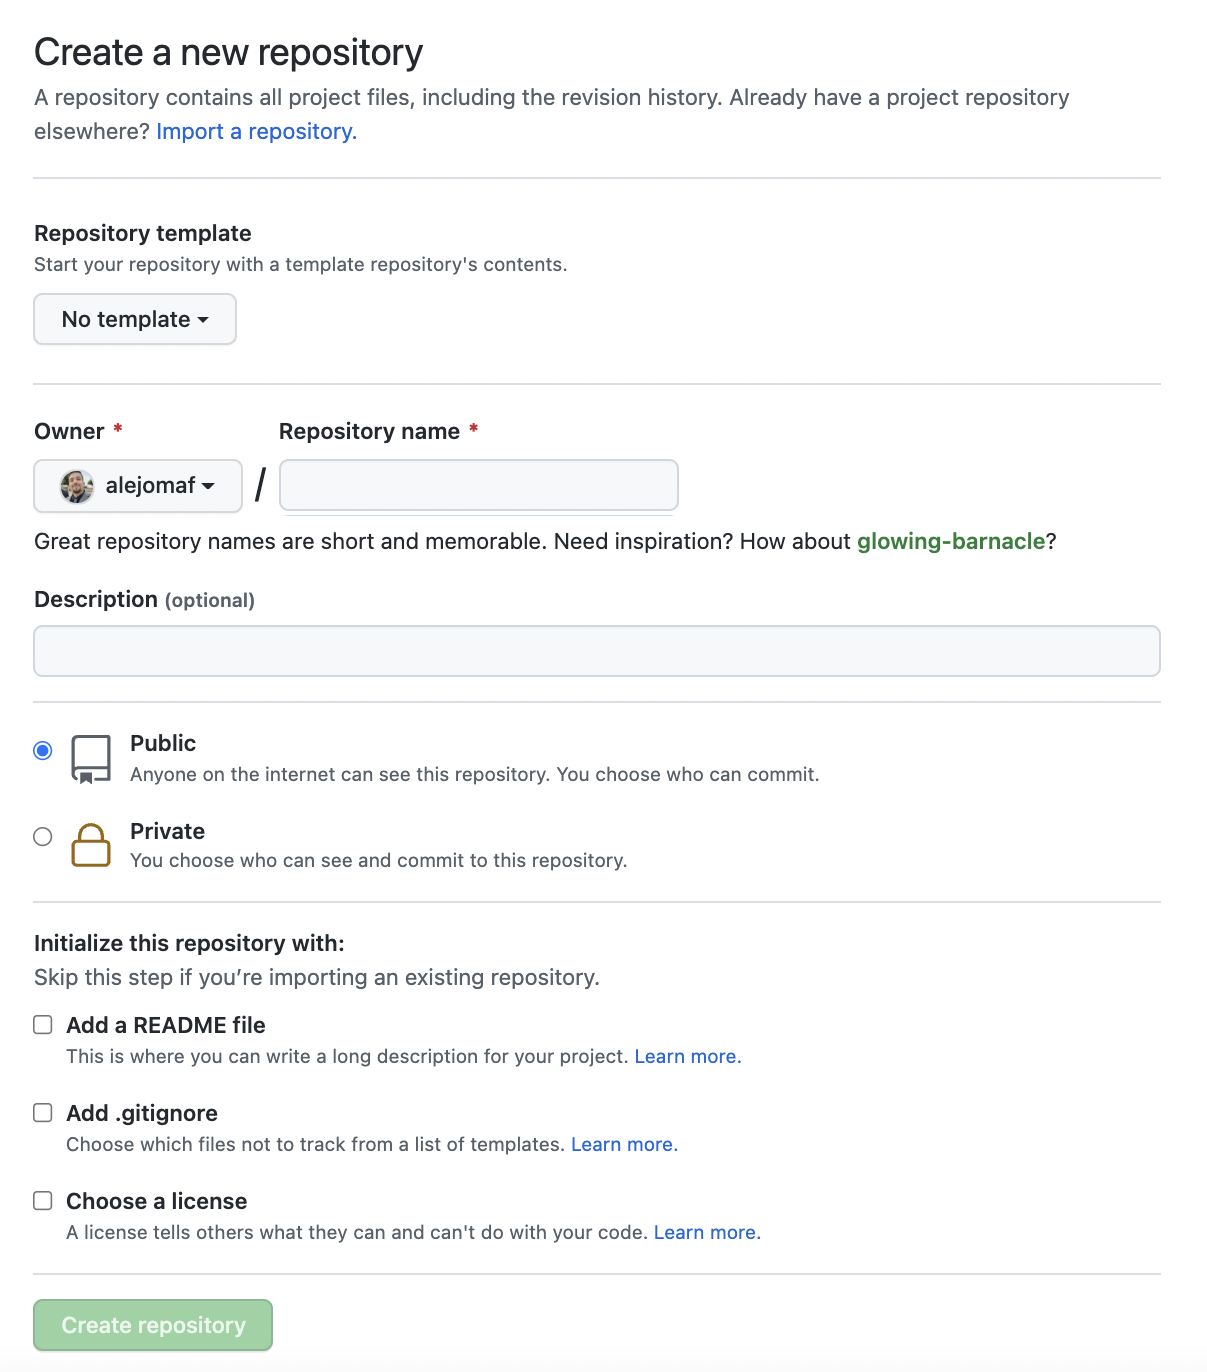
\includegraphics[scale=0.4]{preparacion_entorno/creando_nuevo_repositorio.png}
              \caption{Creando un nuevo repositorio dentro de GitHub}\label{creando_repositorio_github}
          \end{figure}
\end{enumerate}

Con estos sencillos pasos se ha realizado la creación del repositorio del proyecto.

\subsection{Visual Studio Code y Google Cloud, los mejores amigos}
Hoy en día lo nuevo y a lo que la sociedad se dirige es la nube. Dentro de ella se pretenden que se realicen todos los procesos. La mayoría de herramientas y servicios que se nos ofrece cumplen un modelo de caja negra. Es decir, se puede interactuar con ellos y recibir respuestas pero no puede verse qué procesos ocurren dentro de aquella caja.
\\Por esta razón cada vez se empieza a disponer menos de un software como tal y se empiezan a pasar a servicios en línea. Esto no quiere decir que se dejen de usar programas o aplicaciones móviles. Pero la realidad es que sin internet; la mayoría no funcionaría.
\\Esto presenta desventajas siendo la principal que se depende constantemente de una conexión en línea que puede parecer que está presente en todos sitios pero en lugares remotos de la ciudad, como son los pueblos de montaña, el internet no es el mejor compañero, por decirlo, de una manera.
\\Las ventajas son enormes aunque solo se verán las que implican mayor relevancia para el desarrollo del proyecto.
\\El tener ya un repositorio generado con el proyecto subido dentro de él aporta bastante autonomía ya que puede accederse a él y descargar los datos desde cualquier lugar. Pero, ¿y configurarlo?
\\Aquí viene una problemática que no resuelve un entorno de repositorios. El tener que configurarlo todo cada vez que se quiera trabajar desde un sitio distinto. Esto lo resuelven las máquinas virtuales en la nube. El generar un directorio de trabajo donde poder conectar el Visual Studio Code y olvidarse de preocupaciones.
\\Lo segundo que se ha considerado más importante es el ahorro de memoria tanto de RAM como de disco y de procesos que se origina al hacer esto. No es lo mismo tener que trabajar con un portátil conectado todo el día a un enchufe que poder ir llevándolo contigo durante todo el día por el escaso consumo de batería que tiene. Peor si es una torre, solo puedes trabajar desde un único sitio, con la problemática también de que siempre se te puede ir la luz.
\\Estas ventajas expuesta son las que favorecen al desarrollo del proyecto que es realizado por una única persona, pero ¿y si este se hiciera en un equipo? El poder tener varias personas trabajando en el mismo proyecto, tocando los distintos componentes que se están desarrollando dentro de la aplicación es fantástico.

\subsubsection{Crear una máquina virtual en Google Cloud}
Los pasos para la creación de una máquina virtual son:

\begin{enumerate}
    \item El registro es fácil de realizar ya que la herramienta es propiedad de Google. Se omitirá este paso.
    \item Google Cloud se organiza mediante proyectos. Esto brinda facilidades a la hora de calcular el gasto que se tendrá por el uso de la computación en la nube. Aparte de poder facilitar la búsqueda por cada proyecto que se tenga activo. Se procederá a crear un nuevo proyecto clicando arriba a la izquierda a la derecha del título de la página y posteriormente clicando en nuevo proyecto.
    \item Luego se desplegará la barra lateral de la izquierda y se clicará en el apartado de Compute Engine.
    \item Se pulsará el botón de crear instancia. A la hora de rellenar los parámetros se ha comprobado que no es necesario darle demasiada importancia a la zona o región donde se ubique tu máquina. Esta se conectará con una velocidad bastante decente. En el apartado de configuración de máquina con 2GB de RAM y 1VCPU se tendrán suficientes recursos. El tamaño del disco eligido será de 20GB. Dentro de la sección Firewall se habilitará el tráfico HTTP y HTTPS. Y posteriormente se pulsará en crear.
    \item Después de haber creado la máquina se le asignará una IP estática pública que se usará para conectarse a ella mediante SSH.
    \item En el momento de haber creado la máquina esta ha dado una clave privada SSH para poder conectarse a ella. Es necesario guardarla.
\end{enumerate}

\subsubsection{Configurar claves SSH}

Teniendo ya la clave privada SSH de la máquina virtual se utilizará para realizar la conexión con ella. Pero para ello es necesario configurarla. Hay que acceder al fichero usuario/.ssh/config y añadir tres nuevas líneas:
\begin{verbatim}
    Host "Dirección IP"
    HostName "Nombre del host"
    User "Nombre de usuario"
\end{verbatim}
Lo último que nos queda es realizar la conexión mediante SSH a la máquina con Visual Studio Code.

\subsubsection{Realizar conexión SSH mediante Visual Studio Code}
Dentro del apartado de extensiones de Visual Studio Code se localizarán los siguientes plugins para instalar:

\begin{itemize}
    \item Remote - SSH
    \item Remote - SSH: Editing Configuration Files
\end{itemize}

Luego de la instalación de estas dos extensiones se procederá a realizar la conexión. Abajo a la izquierda aparecerá la opción de poder conectarse mediante SSH. Hay que clicar sobre ella y luego se pulsará en ``Connect to Host'' añadiendo la dirección IP estática pública que dio Google Cloud.
\\Ya con esto estaría la masa del entorno hecha, solo hace falta darle un poco de forma y calor para poder finalizarla.

\subsection{Instalación de las extensiones de Visual Studio Code dentro de la MV}

Esta es la lista de componentes con la que se trabajará en todas las fases del proyecto. Hay que acceder a las extensiones dentro de Visual Studio Code y proceder a instalarlas dentro de la máquina virtual.

\begin{itemize}
    \item Docker
    \item LaTeX
    \item LaTeX Workshop
\end{itemize}

Los complementos de Latex ayudarán más tarde con la redacción del Trabajo de Fin de Grado.
\\En Visual Studio Code también se instalará:

\begin{itemize}
    \item Bootstrap 4 snippets
    \item HTML snippets
    \item CSS snippets
\end{itemize}

\subsection{Configuración de la máquina virtual}

Desde Visual Studio Code se accederá a la terminal de la máquina virtual. Se pinchará en ``Ver'' en la sección superior y luego en Terminal. Desde ahí se podrá controlar la máquina.

\subsubsection{Actualización del sistema}
Se realizará una actualización del sistema para evitar posibles fallos en un futuro:
\begin{verbatim}
    sudo apt-get update
    sudo apt-get upgrade
\end{verbatim}

\subsubsection{Instalación de Node JS}
\begin{verbatim}
    sudo apt install nodejs
\end{verbatim}

\subsubsection{Instalación de Angular 12}
\begin{verbatim}
    sudo npm install npm@latest -g
    sudo npm install -g @angular/cli
\end{verbatim}

\subsubsection{Instalación de Docker y Docker Compose}
\begin{verbatim}
    \\Instalacion de Docker

    sudo apt install apt-transport-https ca-certificates
    curl software-properties-common
    curl -fsSL https://download.docker.com/linux/ubuntu/gpg
    sudo apt-key add -
    sudo add-apt-repository 
    "deb [arch=amd64] https://download.docker.com/linux/ubuntu focal stable"
    sudo apt install docker-ce

    \\Instalacion de Docker Compose

    sudo curl -L "https://github.com/docker/compose/releases/download/1.26.0
    /docker-compose-$(uname -s)-$(uname -m)" -o /usr/local/bin/docker-compose
    sudo chmod +x /usr/local/bin/docker-compose
\end{verbatim}

\subsubsection{Configuración de credenciales de Git e instalación del repositorio}
\begin{verbatim}
    //Configuración de credenciales

    git config --global user.name "tu nombre de usuario"
    git config --global user.email "tu correo electrónico"
    git config --global user.password "tu contraseña"

    //El repositorio se ubicará dentro de la carpeta raíz del usuario
    
    git clone https://github.com/alejomaf/Inventarium.git
\end{verbatim}